\subsection{RAID 1}

RAID 1 es una técnica de almacenamiento cuyo objetivo principal es proporcionar redundancia y alta disponibilidad mediante espejado.

Conceptualmente, cada dato que se escribe en un disco se copia simultáneamente en otro disco. Ambos contienen exactamente la misma información, como se muestra en la figura \ref{fig:raid1}.

\begin{figure}[!ht]
  \centering
  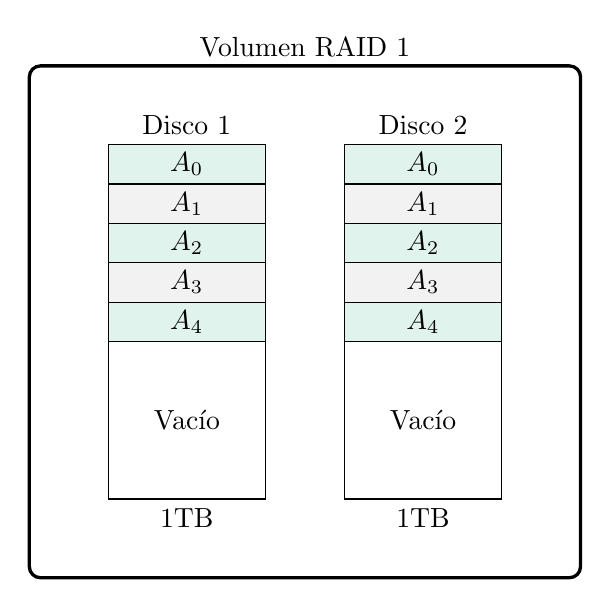
\begin{tikzpicture}
    \node[above] at (1,2.5) {Disco 1};
    \foreach \y\t\c in {
        0/4/white!95!blue!93!green,
        0.5/3/gray!10,
        1/2/white!95!blue!93!green,
        1.5/1/gray!10,
        2/0/white!95!blue!93!green}{
      \draw[fill=\c] (0,\y) rectangle node{\(A_\t\)} (2,{0.5+\y});
    }
    \draw (0,0) rectangle node{Vacío} (2,-2);
    \node[below] at (1,-2) {1TB};

    \node[above] at (4,2.5) {Disco 2};
    \foreach \y\t\c in {
        0/4/white!95!blue!93!green,
        0.5/3/gray!10,
        1/2/white!95!blue!93!green,
        1.5/1/gray!10,
        2/0/white!95!blue!93!green}{
      \draw[fill=\c] (3,\y) rectangle node{\(A_\t\)} (5,{0.5+\y});
    }
    \draw (3,0) rectangle node{Vacío} (5,-2);
    \node[below] at (4,-2) {1TB};

    \draw[very thick,rounded corners] (-1,-3) rectangle (6,3.5);
    \node[above] at (2.5,3.5) {Volumen RAID 1};
  \end{tikzpicture}
  \caption{Tamaño del volumen de RAID 1: 1TB.}
  \label{fig:raid1}
\end{figure}
Si uno de los discos falla, el otro sigue conteniendo una copia completa de todos los datos, por lo que el sistema puede continuar funcionando sin pérdida de información.

\paragraph{Ventajas:}
\begin{itemize}
  \item Alta tolerancia a fallos: soporta la falla de un disco (en un arreglo de dos discos).
  \item Recuperación sencilla: basta con reemplazar el disco averiado y reconstruir la copia.
  \item Las lecturas pueden ser más rápidas, ya que el sistema puede leer desde cualquiera de los discos.
\end{itemize}

\paragraph{Desventajas:}
\begin{itemize}
  \item La capacidad útil es solo la de un disco, ya que la otra mitad se utiliza para la copia.
  \item Las escrituras deben realizarse en todos los discos del espejo, por lo que el rendimiento de escritura no mejora significativamente.
\end{itemize}

\paragraph{Ejemplo}
Si se tienen dos discos de 1 TB la capacidad física total sigue siendo de 2 TB, pero la capacidad útil es de 1 TB. Sin embargo si uno de los discos falla, el sistema sigue funcionando con el otro disco y no se pierde información.

\subsubsection{RAID 1 + Hot Spare}

El Hot Spare (o disco de reserva en caliente) es un disco adicional que no almacena datos mientras el arreglo RAID funciona normalmente, sino que permanece disponible para reemplazar automáticamente a un disco que falle.

A modo de ejemplo, se supone un RAID 1 con dos discos y un Hot Spare, como se muestra en la figura \ref{fig:raid1spare}

\begin{figure}[!ht]
  \centering
  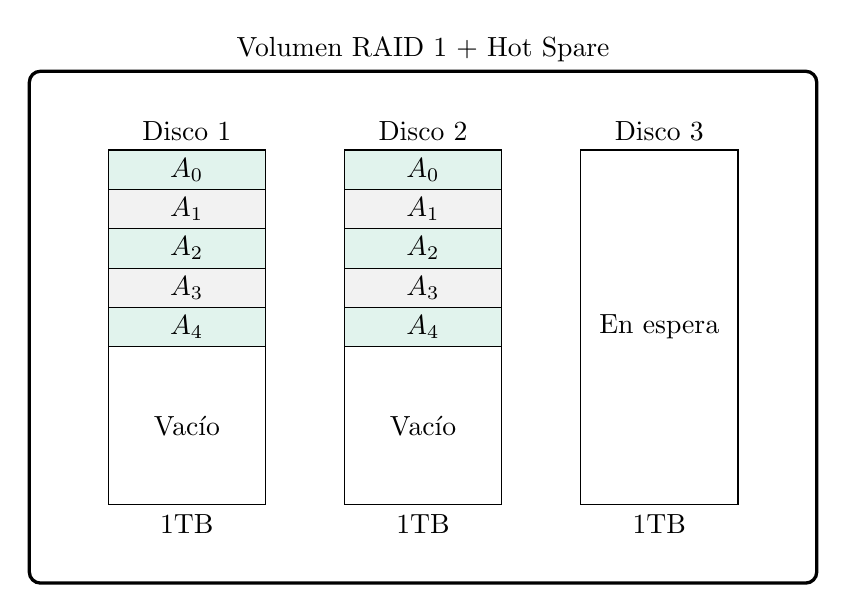
\begin{tikzpicture}
    \node[above] at (1,2.5) {Disco 1};
    \foreach \y\t\c in {
        0/4/white!95!blue!93!green,
        0.5/3/gray!10,
        1/2/white!95!blue!93!green,
        1.5/1/gray!10,
        2/0/white!95!blue!93!green}{
      \draw[fill=\c] (0,\y) rectangle node{\(A_\t\)} (2,{0.5+\y});
    }
    \draw (0,0) rectangle node{Vacío} (2,-2);
    \node[below] at (1,-2) {1TB};

    \node[above] at (4,2.5) {Disco 2};
    \foreach \y\t\c in {
        0/4/white!95!blue!93!green,
        0.5/3/gray!10,
        1/2/white!95!blue!93!green,
        1.5/1/gray!10,
        2/0/white!95!blue!93!green}{
      \draw[fill=\c] (3,\y) rectangle node{\(A_\t\)} (5,{0.5+\y});
    }
    \draw (3,0) rectangle node{Vacío} (5,-2);
    \node[below] at (4,-2) {1TB};

    \node[above] at (7,2.5) {Disco 3};
    \draw (6,2.5) rectangle node{En espera} (8,-2);
    \node[below] at (7,-2) {1TB};

    \draw[very thick,rounded corners] (-1,-3) rectangle (9,3.5);
    \node[above] at (4,3.5) {Volumen RAID 1 + Hot Spare};
  \end{tikzpicture}
  \caption{RAID 1 con Hot Spare. Tamaño final 1TB.}
  \label{fig:raid1spare}
\end{figure}

Si falla el Disco 1:
\begin{enumerate}
  \item El controlador RAID detecta la falla.
  \item Marca el Disco 1 como averiado.
  \item Incorpora automáticamente el Hot Spare al arreglo.
  \item Reconstruye los datos copiándolos desde el Disco 2 al Hot Spare.
\end{enumerate}
El resultado es:
\begin{itemize}
  \item Disco 1: Averiado
  \item Disco 2: Datos
  \item Disco 3: Nueva copia (antes era Hot Spare)
\end{itemize}
Una vez reemplazado físicamente el disco averiado, este puede configurarse como el nuevo Hot Spare.

\begin{table}[!ht]
  \centering
  \begin{tabular}{l|c}
    Cantidad de discos mínima & 2 \\\hline
    Cantidad de discos que pueden fallar & 1 \\ \hline
    Velocidad de escritura relativa a un disco & VDisco~[MB/s] \\\hline
    Velocidad de escritura ponderada & 5 \\ \hline
    Velocidad de lectura relativa a un disco & VDisco~[MB/s] \\ \hline
    Velocidad de lectura ponderada & 5 \\ \hline
    Costo & Medio
  \end{tabular}
  \caption{Características del RAID 1.}
\end{table}
